\documentclass[11pt, twoside, a4paper]{book}

\usepackage{graphicx}
\usepackage[utf8]{inputenc}
\usepackage{ngerman}
%\usepackage{lineno}
\usepackage{verbatim}
\usepackage[squaren]{SIunits}
\usepackage{amsmath}
\usepackage{amsfonts}
\usepackage{amssymb}
\usepackage{enumitem}
\usepackage{fancyhdr}
\usepackage{textcomp}
\usepackage{subcaption}
\usepackage[noadjust]{marginnote}
\usepackage{tikz}
\usepackage{nicefrac}
\usepackage{framed}
\usepackage{import}

\usetikzlibrary{calc,intersections}
\usetikzlibrary{arrows}
\usetikzlibrary{decorations.markings}
\usetikzlibrary{decorations.pathreplacing}
\usepackage[european resistors]{circuitikz}
\usepackage[ 
    top=2cm, 
    bottom=2cm, 
    outer=3cm, 
    inner=3cm,
    marginparwidth=2.5cm,
		headheight=14pt
  ]{geometry}

\usepackage{parskip}
\usepackage{pdfpages}

\setlength{\parindent}{0pt}

\newcommand{\experimentheader}[4]
{
  \iftutor{{\bf Schwierigkeitsgrad:} #1\\}
  \iftutor{{\bf Dauer:} #2\\}
  {\bf Ger\"ate:} #3\\
  {\bf Bauteile:} #4
}

\newcommand{\hintboxNone}{0}
\newcommand{\hintboxExclamation}{1}
\newenvironment{hintbox}[4][\hsize]
{
  \def\FrameCommand
  {%
    {\color{#3}\vrule width 3pt}%
    \hspace{0pt}%must no space.
    \fboxsep=\FrameSep\colorbox{#4}%
  }%
  \MakeFramed{\hsize#1\advance\hsize-\width\FrameRestore}%
  \mbox{\textbf{#2}:}%
}
{
  \endMakeFramed
}
\newcommand{\xhintbox}[3]
{
  \begin{hintbox}{Achtung}{red!50}{red!10}
    #3
  \end{hintbox}
}

\newenvironment{hint}
{
  \begin{hintbox}{Hinweis}{green!50}{green!10}
}
{
  \end{hintbox}
}

\newenvironment{definition}
{
  \begin{hintbox}{Definition\\}{white!50}{white!10}
}
{
  \end{hintbox}
}

\newenvironment{important}
{
  \begin{hintbox}{Hinweis}{gray!50}{gray!10}
}
{
  \end{hintbox}
}

\newenvironment{jason}
{
  \begin{hintbox}{Achtung}{red!50}{red!10}
}
{
  \end{hintbox}
}

\newcommand{\mandatoryenumi}
{
  \renewcommand{\labelenumi}{\arabic{enumi}.} 
}
\newcommand{\optionalenumi}
{
  \renewcommand{\labelenumi}{$\bigstar$\quad\arabic{enumi}.} 
}
\newcommand{\mandatoryenumii}
{
  \renewcommand{\labelenumii}{(\alph{enumii})} 
}
\newcommand{\optionalenumii}
{
  \renewcommand{\labelenumii}{$\bigstar$\quad(\alph{enumii})} 
}
\newcommand{\icname}[1]{\mbox{\tt #1}}


  %\newcommand{\iftutor}[1]{}
\newcommand{\ifnotutor}[1]{#1}

  \newcommand{\iftutor}[1]{#1}
\newcommand{\ifnotutor}[1]{}


\newenvironment{tutorhint}{\comment}{\endcomment}
\newenvironment{todo}{\comment}{\endcomment}
\newenvironment{solution}{\comment}{\endcomment}
\iftutor
{
  \renewenvironment{todo}
  {
    \hintbox{Todo}{red!50!yellow!90}{red!50!yellow!20}
  }
  {
    \endhintbox
  }
  \renewenvironment{tutorhint}
  {
    \hintbox{Tutorenhinweis der Stunde}{blue!50}{blue!10}
  }
  {
    \endhintbox
  }
  \renewenvironment{solution}
  {
    \hintbox{L\"osung}{black!80}{black!5}
  }
  {
    \endhintbox
  }
}
\newcommand{\etutorhint}[1]
{
  \iftutor{
    \tutorhint
      #1
    \endtutorhint
  }
}
\newcommand{\esolution}[1]
{
  \iftutor
  {
    \solution
    #1
    \endsolution
  }
}
\newcommand{\etodo}[1]
{
  \iftutor
  {
    \todo
    #1
    \endtodo
  }
}



\begin{document}

\renewcommand{\thechapter}{\arabic{chapter}}
\setcounter{chapter}{19}
\def\chaptername{Versuch}

\chapter{Molare Wärmekapazität von Luft}
\label{v:6}

\etodo{\textbf{Praktikumsleitung:} Nach Versuchsende sicherstellen, dass die Ventile an den Zylindern offen sind. Ansonsten wird, durch das Zusammenziehen beim Abkühlen der Luft im Zylinder, Wasser aus dem U-Rohr in den Zylinder gesaugt, welches mit der Zeit den Heizdraht korrodiert.}

Im Versuch soll die Wärmekapazität eines Gases (hier: Luft) bestimmt werden.

%------------------------------------------------
\section{Stichworte}
%------------------------------------------------

Allgemeine Gasgleichung; molare Wärmekapazitäten $C_P$ und $C_V$; 1. Hauptsatz der Thermodynamik; Energie des geladenen Kondensators
%
%------------------------------------------------
\section{Literatur}
%------------------------------------------------

Gehrtsen, Kapitel 5.1.5 und 5.2.2 bis 5.2.4
%
%------------------------------------------------
\section{Anwendungsbeispiele}
%------------------------------------------------
%
In jeder Beschreibung von chemischen Prozessen fester, flüssiger oder gasförmiger Stoffe spielt die Thermodynamik eine herausragende Rolle. Sie wird deshalb im Studium der Chemie und Biologie ausführlicher an anderer Stelle eingeübt. Ein Gesichtspunkt soll hier genauer untersucht werden: Eine große Anzahl von Maschinen und Motoren nutzt die Expansion von Gasen aus, um einen Kolben zu bewegen (früher in Dampfmaschinen, heute in den Explosionsmotoren der Autos), Stichwort Pneumatik.

%Energieäquivalenzen, kinetische Gastheorie, Carnot'scher Kreisprozess.
%
%------------------------------------------------
\section{Theoretischer Hintergrund}
%------------------------------------------------

\subsection{Die Zustandsgleichung idealer Gase}

Die Zustandsgleichung eines Systems gibt an, wie seine messbaren Eigenschaften voneinander abhängen. Der Zustand einer Gasmasse $M$ wird durch drei Größen volständig beschrieben: Temperatur $T$, Druck $p$ und Volumen $V$. Zwei davon können unabhängig voneinander variiert werden, die dritte ist dann eindeutig bestimmt. Dieser Zusammenhang ist gegeben durch die \textit{allgemeine Gasgleichung}:
\begin{equation}
	pV = Nk_bT = \nu RT.
\end{equation}
Hierbei ist $N$ die Anzahl von Molekülen in der Gasmasse, $\nu$ beschreibt die Menge des Gases in mol. Die Gaskonstante ist definiert als: $R = N_A k_b = 8,31\, \mathrm{J\, K^{-1}\, mol^{-1}}$.\\
Diese Gasgleichung gilt, aufgrund ihrer Herleitung, eigentlich nur für \textit{ideale Gase}, in denen Teilchen abgesehen von kurzzeitigen Stößen keine Kräfte aufeinander ausüben und selbst kein messbares Eigenvolumen haben. Viele reale Gase verhalten sich allerdings relativ ähnlich zu einem idealen Gas, so dass auch hier die Gasgleichung als Näherung benutzt werden kann.

Folgerungen aus der Gasgleichung sind
\begin{itemize}
	\item das \textit{Gesetz von Boyle-Mariotte}: Bei konstanter Temperatur ist der Druck umgekehrt proportional zum Volumen: $\mathrm{p\sim V^{-1} \quad (T=const.)}$
	\item das \textit{Gesetz von Gay-Lussac}: Bei konstantem Volumen steigt der Druck mit der Temperatur: $\mathrm{p\sim T \quad (V=const.)}$
	\item das \textit{Gesetz von Charles} (oft auch nach \textit{Gay-Lussac} benannt: Bei konstantem Druck steigt das Volumen wie die Temperatur: $\mathrm{V\sim T \quad (p=const.)}$
\end{itemize}

\subsection{Der 1. Hauptsatz der Wärmelehre}

Der erste Hauptsatz der Thermodynamik, der nur eine Umformulierung des Energieerhaltungssatzes ist, beschreibt, was passiert wenn man einem System von außen Wärmeenergie zuführt:\\
\textit{Die Wärmeenergie $\Delta Q$ wird teilweise in mechanische Arbeitsleistung $\Delta W$ verbraucht. Der Rest von $\Delta Q$ führt zu einer Steigerung der inneren Energie $U$ des Systems um $\Delta U$:}
%\begin{important}
	\begin{equation}
		\Delta Q = \Delta U + \Delta W
	\end{equation}
%\end{important}

Bei idealen Gasen entspricht die innere Eneregie der Bewegungsenergie der Moleküle, ist also proportional zur Temperatur des Gases (s. Gleichung \ref{eq:spez_Waermekapazitaet}). Die mechanische Arbeitsleistung besteht aus der Druckarbeit $\Delta W = p\,\Delta V$. Für ein Gas lautet also der Energieerhaltungssatz:
\begin{equation} \label{eq:ersterHauptsatz}
	dQ = dU + p\,dV
\end{equation}
Hierbei bezeichnen $dQ$, $dU$ und $dV$ infinitesimale Änderungen der jeweiligen Größen, sie sind also die Verallgemeinerung der vorher betrachteten großen Änderungen $\Delta Q$, $\Delta U$ und $\Delta V$.

\subsection{Die molare Wärmekapazität von Luft}

Wie man aus Gleichung \ref{eq:spez_Waermekapazitaet} sieht, ist die molare Wärmekapazität von Luft definiert als
\begin{equation}
	C_{mol} = \frac{1}{n}\frac{dQ}{dT},
\end{equation}
wobei $n$ die Gasmenge in mol angibt.\\
Unter isochoren Bedingungen ($dV = 0$) kann man diese Definition, unter Benutzung von Gleichung \ref{eq:ersterHauptsatz}, umschreiben zu
\begin{equation}
	C_V = \frac{1}{n}\frac{dU}{dT}.
\end{equation}
$C_V$ steht dabei für die molare Wärmekapazität bei konstantem Druck: $C_V \hat{=} C_{mol}(p=const.)$\\
Dies lässt sich mit der Dulong-Petite'schen Regel (s. Gleichung \ref{eq:Dulong-Petit}) und der Gaskonstanten $R$ schreiben als
\begin{equation}
	C_V = \frac{f}{2}R.
\end{equation}

\begin{tutorhint}
%------------------------------------------------
\section{Fragen zur Vorbereitung}
%------------------------------------------------

\begin{enumerate}
 %
% \item Was soll heute im Praktikum gemessen werden? Warum?
 %
 \item Wie lautet das ideale Gasgesetz? Welche Einschränkungen liegen ihm zugrunde?
 %
 \item Was und wie gross ist R (mit Einheit) ?
 %
 \item Wie ist die Temperaturskala definiert? (Umrechnung Kelvin in Celsius)
 %
 \item Was für Bewegungsmöglichkeiten haben Moleküle in Gasen?
 %
 \item Welche Unterscheidung muss bei der Betrachtung der Wärmekapazität bei Gasen gemacht werden? Warum ist das bei Festkörpern nicht nötig?
 %
 \item In welchem Zusammenhang stehen $c_v$ und $c_p$ im Fall von idealen Gasen?
 %
 \item Wie stehen die Bewegungsmöglichkeiten mit den Freiheitsgraden in Zusammenhang?
 %
 \item Wie hängt $c_v$ mit den Freiheitsgraden zusammen?
 %
 \item Wie wird $c_v$ von Luft im Praktikum bestimmt?
 %
\end{enumerate}
\end{tutorhint}

%------------------------------------------------
\section{Durchführung} 
%------------------------------------------------

Die Luft befindet sich in einem Plexiglaszylinder (dessen Innen-Volumen man durch Ausmessen bestimmen kann). Sie wird kurzzeitig durch einen Draht erhitzt. Im Gas erhöht sich der Druck, der in einem Wassermanometer die Wassersäule ansteigen lässt. Das kann man beobachten und ausmessen. Die Energie, mit der man den Heizdraht erhitzt, kommt aus einem Kondensator, der mit verschieden hoher Spannung aufgeladen werden kann.\\
Man heizt also die Luft in einem bekannten, konstanten Volumen auf verschiedene Temperaturen auf und misst den dazugehörigen Druckanstieg.\\

\underline{Zubehör:} Zylinder mit Heizdraht und Wassermanometer, Gleichspannungsquelle mit Potentiometer und Voltmeter (0 - 600 Volt), Kondensator, Messlatte.

\begin{enumerate}
 %
 \item Messen Sie jeweils drei Mal die Ausdehnung der Luft bei Erwärmung, für Ladespannungen am Kondensator von 150\;V bis 500\;V in Schritten von 50\;V nach dem folgenden Rezept: 
  \begin{itemize}
	 \item Stellen Sie die Spannung am Kondensator ein. Verschliessen Sie das enge Rohr des Wassermanometers mit einem Finger.
	 \item Messen Sie den maximalen Ausschlag des Manometers, wenn Sie nun den Kondensator mit Hilfe des Tasters entladen und damit die Luft erwärmen.
	 \item Entfernen Sie den Finger vom Manometer, damit sich Druck und Temperatur im Messzylinder ausgleichen können.
	 \item Wiederholen Sie diese Messung noch zwei Mal, bevor Sie zur nächsten Spannung übergehen.
	\end{itemize}
 %
 \item Messen Sie zum Abschluss die Innenmaße des Zylinders (Länge und Durchmesser), um das Luftvolumen berechnen zu können. Wie groß ist die Messungenauigkeit?
 %
\end{enumerate}

%------------------------------------------------
\section{Auswertung} 
%------------------------------------------------
\etodo{Musterauswertung.\\
Misst man hier nicht eigentlich $c_p$?}

Benutzen Sie für die Auswertung folgende Angaben:
\begin{table}[h]
		\begin{tabular}{ll}
			Kapazität des Kondensators & $C = 20\,\mu$F \\
			Avogadrozahl & $N_A = 6,022\cdot 10^{23}\,\mathrm{mol}^{-1}$
		\end{tabular}
\end{table}

\noindent
Die Radien der beiden Schenkel des Wassernanometers verhalten sich wie $r_1$ : $r_2$ =1 : 4,5.

\begin{enumerate}
 %
 \item Berechnen Sie das Volumen $V$ des Zylinders inklusive seines Fehlers.
 %
 \item \label{v6:Graph} Tragen Sie den Mittelwert des maximalen Ausschlags $h_1$ am Wassermanometer graphisch gegen das Quadrat der Kondensatorspannung $U$ auf.
 %
 \item Berechnen Sie die molare Wärmekapazität $C_V$ von Luft aus der Steigung der Geraden $h_1 = f(U^2)$. Benutzen Sie die Beziehung
  \begin{equation}
	 h_1 = const\cdot \frac{1}{C_V}U^2\; .  
  \end{equation}
 Leiten Sie die Formel her und berechnen Sie die Konstante
  \begin{equation}
   const = \frac{R\cdot C}{\rho\cdot g\cdot V\cdot 1,05\cdot 2}\; .
  \end{equation} 
	%
	\begin{solution}
		\etodo{Herleitung streichen? Oder Hinweise: Bild des U-Rohrs, ideales Gasgesetz, Energie des geladenen Kondensators, $\Delta p\propto \Delta h$,...}
		Ansatz: Die im Kondensator gespeicherte Energie wird in Wärme umgewandelt
		\begin{align*}
			E_{el} &= \Delta Q\\
			\frac{1}{2}CU^2 &= \Delta T\cdot C_V\cdot n
		\end{align*}
		\begin{equation}\label{eq:C_V1}
			\Leftrightarrow C_V = \frac{CU^2}{2n\Delta T}
		\end{equation}
		Die Temperaturdifferenz bekommen wir aus dem idealen Gasgesetz. Es gilt
		\begin{align*}
			pV &= nRT\quad\mathrm{vor\, dem\, Strompuls}\\
			\left( p+\Delta p\right) V &= nR\left(T+\Delta T\right)\quad\mathrm{direkt\, danach}
		\end{align*}
		%
		Setzen wir $\Delta pV=nR\Delta T$ in Gleichung \ref{eq:C_V1} ein und kürzen $n$ weg, so bekommen wir
		\begin{equation}\label{eq:C_V2}
			C_V=\frac{CU^2R}{2\Delta pV}
		\end{equation}
		%
		\begin{minipage}{.3\textwidth}
			\begin{center}
				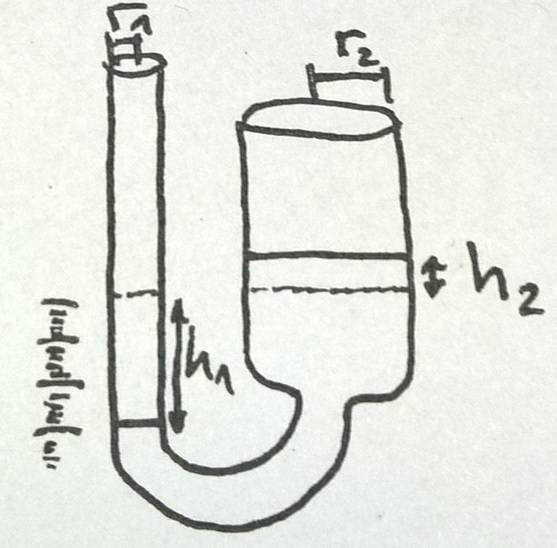
\includegraphics[width=0.90\textwidth]{Abbildungen/URohr_Bea.jpg}
			\end{center}
		\end{minipage}
		%
		\begin{minipage}{.6\textwidth}
			Es gilt
			\begin{equation}\label{eq:Delta_p}
				\Delta p = \rho g \cdot\Delta h,
			\end{equation}
			wobei $\Delta h$ die Gesamthöhe der Wassersäule ist: $\Delta h = h_1+ h_2$.\\
			$h_1$ wurde gemessen, $h_2$ ergibt sich über das Volumen in beiden Schenkeln des U-Rohrs:
			\begin{align*}
				V &= \pi r_1^2 h_1 = \pi r_2^2 h_2\\
				\Leftrightarrow h_2 &= h_1\cdot\left(\frac{r_1}{r_2}\right)^2 = h_1\cdot\left(\frac{1}{4,5}\right)^2\\
				\Rightarrow \Delta h &= 1,05 h_1
			\end{align*}
		\end{minipage}
		%
		Einsetzen in Gleichung \ref{eq:Delta_p} und dann in Gleichung \ref{eq:C_V2} ergibt
		\begin{align}
			C_V &= \frac{CU^2 R}{2V\rho g\cdot 1,05h_1}\\
			\Leftrightarrow h_1 &= \frac{RC}{\rho gV\cdot 2\cdot 1,05}\cdot\frac{U^2}{C_V}
		\end{align}
	\end{solution}
 %
 \item Schätzen Sie den Fehler von $C_V$ aus der Grenzgeraden der Auftragung aus \ref{v6:Graph} sowie dem Fehler des Volumens ab.
 %
 \item Berechnen Sie die Boltzmann Konstante $k$ (mit Fehler) aus der Beziehung
  \begin{equation}
   C_V = \frac{5}{2}k\cdot N_A \; .
  \end{equation}
  %
\end{enumerate}

\end{document}